\documentclass[11pt]{article}
\usepackage{mathpartir}
\usepackage{pifont}
\usepackage{multicol}
\usepackage{listings}
\usepackage{pgf}
\usepackage{tikz}
\usepackage{alltt}
\usepackage{hyperref}
\usepackage{url}
\usepackage{amsmath}
\usepackage{amssymb}
\usepackage{dafny}
\usepackage{fancyvrb}
\usetikzlibrary{arrows,automata,shapes,positioning}
\tikzstyle{block} = [rectangle, draw, fill=blue!20, 
    text width=5em, text centered, rounded corners, minimum height=2em]
\tikzstyle{bt} = [rectangle, draw, fill=blue!20, 
    text width=1em, text centered, rounded corners, minimum height=2em]
\newcommand{\xmark}{\ding{55}}

\newtheorem{defn}{Definition}
\newtheorem{crit}{Criterion}
\newcommand{\true}{\mbox{\sf true}}
\newcommand{\false}{\mbox{\sf false}}

\newcommand*\circled[1]{\tikz[baseline=(char.base)]{
            \node[shape=circle,draw,inner sep=2pt] (char) {#1};}}


\newcommand{\handout}[5]{
  \noindent
  \begin{center}
  \framebox{
    \vbox{
      \hbox to 5.78in { {\bf Software Testing, Quality Assurance and Maintenance } \hfill #2 }
      \vspace{4mm}
      \hbox to 5.78in { {\Large \hfill #5  \hfill} }
      \vspace{2mm}
      \hbox to 5.78in { {\em #3 \hfill #4} }
    }
  }
  \end{center}
  \vspace*{4mm}
}

\newcommand{\lecture}[4]{\handout{#1}{#2}{#3}{#4}{Lecture #1}}
\topmargin 0pt
\advance \topmargin by -\headheight
\advance \topmargin by -\headsep
\textheight 8.9in
\oddsidemargin 0pt
\evensidemargin \oddsidemargin
\marginparwidth 0.5in
\textwidth 6.5in

\parindent 0in
\parskip 1.5ex
%\renewcommand{\baselinestretch}{1.25}

\usepackage{enumitem}

\newtheorem{prop}{Proposition}
\newtheorem{lemma}{Lemma}
\usepackage{ebproof}
\newcommand{\qedsymbol}{\rule{1ex}{1ex}}
\newcommand{\sem}[3]{\langle #1, #2 \rangle \Downarrow #3}

\lstset{ %
language=Java,
basicstyle=\ttfamily,commentstyle=\scriptsize\itshape,showstringspaces=false,breaklines=true,numbers=left}

%\usepackage{fontspec}
%\setmonofont{Cousine}[Scale=MatchLowercase]

\begin{document}

\lecture{17 --- March 31, 2025}{Winter 2025}{Patrick Lam}{version 1}

We are still pretty confident in our bubble sort implementation. We did, however, use multisets.
This is not a correctness issue, but it's good to know how to implement things ourselves.


\section*{Using sequences rather than multisets}
We are instead going to use sequences, which we briefly mentioned in Lecture 16. As we (briefly) saw back there,
Dafny can seamlessly convert arrays into sequences; we'll use sequences in our lemmas.
A Dafny $\mathsf{seq}\langle T \rangle$ is an immutable sequence of elements of type $T$;
for example, $\mathsf{seq}\langle \mathsf{int} \rangle$ is a sequence of \textsf{int}s. Unlike arrays and lists,
but more like a Java String, they are immutable. Recall that if `a' is an array then `a[..]' is a sequence
with the contents of the array.

Let's start with some helper functions. Note that since a \textsf{seq} is a functional datatype, we can't
modify it, but we can easily take a sub-sequence with \textsf{a[1..]}.
\begin{lstlisting}[language=dafny]
/**
  Returns number of occurrences of a given value `val` inside a given sequence
 */
function count(a:seq<int>, val:int): nat
{
  if |a| == 0 then 0
  else
    if a[0] == val then 1 + count(a[1..], val)
    else count(a[1..], val)
}
\end{lstlisting}
Dafny knows that this function terminates---the length of \textsf{count} is decreasing in recursive calls.

We use this function to define a predicate which says whether \textsf{a} is a permutation of \textsf{b}---recall
that this was the main problem in our incomplete specification of bubble sort.
\begin{lstlisting}[language=dafny]
/**
  A sequence `b` is a permutation of sequence `a` if every integer `v` has
  exactly the same number of occurrences in `a` and in `b`
 */
ghost predicate perm(a: seq<int> , b:seq<int>)
{
  forall v :: count(a, v) == count(b, v)
}
\end{lstlisting}
Dafny complains that \textsf{perm} is not compilable unless we label it a \textsf{ghost} predicate, which means
that we can use it in specifications but not in code. That's all we need anyway.

We know some things about permutation. Dafny can figure them out, but we help it by expressing them.
\begin{lstlisting}[language=dafny]
/** Permutation is transitive.
    Dafny can prove that automatically.
 */
lemma trans_perm(a:seq<int>, b:seq<int>, c:seq<int>)
  requires perm(a, b) && perm(b, c)
  ensures perm(a, c)
{}

/** Permutation is commutative.
    Dafny can prove that automatically.
  */
lemma comm_perm(a:seq<int> , b:seq<int> )
  requires perm(a, b)
  ensures perm(b, a)
{}
\end{lstlisting}

%% There are other things Dafny can prove about permutations. We didn't say that if
%% \textsf{perm(a,b)} then $|\mathsf{a}| = |\mathsf{b}|$ but Dafny can prove it automatically:
%% \begin{lstlisting}[language=dafny]
%% /** Permutation is transitive.
%%     Dafny can prove that automatically.
%%  */
%% lemma same_size(a:seq<int>, b:seq<int>)
%%   requires perm(a, b)
%%   ensures |a| = |b|
%% {}
%% \end{lstlisting}

Here's a lemma about swapping two positions in a sequence. Dafny cannot prove it automatically.
I'll leave this as an exercise.

\begin{lstlisting}[language=dafny]
/**
   If sequences `a` and `b` differ only in two positions, and the values in
   these to positions are swapped, then sequences are permutations of one
   another.

   This is assumed without a proof. Completing the proof is left as an exercise.
 */
lemma swap_lemma(a: seq<int>, b:seq<int>, pos1:nat, pos2:nat)
  requires |a| == |b|
  requires 0 <= pos1 < pos2 < |a|
  requires forall k :: 0 <= k < |a| && k != pos1 && k != pos2 ==> a[k] == b[k]
  requires a[pos1] == b[pos2]
  requires a[pos2] == b[pos1]
  ensures perm(a, b)
  { assume(false); }
\end{lstlisting}

We use the following method in our bubble sort. Here we specify it in isolation:
\begin{lstlisting}[language=dafny]
/** A helper method to swap two positions in an array */
method swap(a: array<int>, pos1:nat, pos2:nat)
  modifies a
  requires 0 <= pos1 < pos2 < a.Length
  ensures forall k :: 0 <= k < a.Length && k != pos1 && k != pos2 ==> a[k] == old(a[k])
  ensures a[pos1] == old(a[pos2])
  ensures a[pos2] == old(a[pos1])
{
  var temp := a[pos2];
  a[pos2] := a[pos1];
  a[pos1] := temp;
}
\end{lstlisting}

Now here is an implementation of bubble sort using the helper method and the lemmas.
We do a lot of the work for Dafny here---Dafny doesn't know these properties of permutations
by default.
\begin{lstlisting}[language=dafny]
/**
   Verified version of bubble sort, in which the prove that the output is
   permutation of the input is done explicitly without using any special help
   from Dafny.
 */
method bubbleSort3 (a: array<int>)
  requires a.Length > 0
  ensures forall u, v :: 0 <= u < v < a.Length ==> a[u] <= a[v]
  ensures perm(a[..], old(a[..]))
  modifies a
{
  var i:nat := 1;

  while (i < a.Length)
    invariant i <= a.Length
    invariant forall u, v :: 0 <= u < v < i ==> a[u] <= a[v]
    invariant perm(a[..], old(a[..]))
  {
    var j:nat := i;
    while (j > 0)
      invariant 0 <= j <= i
      invariant forall u, v :: 0 <= u < v < j ==> a[u] <= a[v]
      invariant forall u, v :: 0 <= u < j < v <= i ==> a[u] <= a[v]
      invariant forall u, v :: j <= u < v <= i ==> a[u] <= a[v]
      invariant perm(a[..], old(a[..]))
    {
      ghost var old_a := a[..];
      if (a[j-1] > a[j]) {
        // Swap a[j-1] and a[j]
        swap(a, j-1, j);
        swap_lemma(old_a, a[..], j-1, j);
        comm_perm(old_a, a[..]);
      }
      j := j - 1;

      trans_perm(a[..], old_a, old(a[..]));
      assert(perm(a[..], old(a[..])));
    }
    i := i+1;
  }
}
\end{lstlisting}
Here we add the postcondition we were missing before in our na\"ive
initial try. The invariants are also similar to the previous
non-refactored example, except that we use \textsf{perm} instead of
the multisets that we had invoked before. The swap operation itself, though,
also uses the \textsf{swap\_lemma} and the commutativity property
\textsf{comm\_perm}. Finally, we also point out to Dafny that \textsf{perm} is
transitive at the end of the outer loop.

It turns out, though, that Dafny actually only really needs the
\textsf{swap\_lemma}.

\section*{Bounding runtimes}
Dafny can do that too: it can prove that this bubble sort implementation is
$O(|a|^2)$. We add some instrumentation to our earlier implementation and assert
on the instrumentation's values.

\begin{lstlisting}[language=dafny]
method bubbleSort4 (a: array<int>)
  requires a.Length > 0
  ensures forall u, v :: 0 <= u < v < a.Length ==> a[u] <= a[v]
  modifies a
{
  // counter that counts number of executions of the main loop
  var cnt := 0;
  var i:nat := 1;

  while (i < a.Length)
    invariant i <= a.Length
    invariant forall u, v :: 0 <= u < v < i ==> a[u] <= a[v]
    invariant cnt <= a.Length * i
  {
    var j:nat := i;
    while (j > 0)
      invariant 0 <= j <= i
      invariant forall u, v :: 0 <= u < v < j ==> a[u] <= a[v]
      invariant forall u, v :: 0 <= u < j < v <= i ==> a[u] <= a[v]
      invariant forall u, v :: j <= u < v <= i ==> a[u] <= a[v]
      invariant cnt <= a.Length * i + (i-j)
    {
      if (a[j-1] > a[j]) {
        // Swap a[j-1] and a[j]
        var temp := a[j-1];
        a[j] := temp;
        a[j-1] := a[j];
      }
      j := j - 1;
      // increment count each iteration of the loop
      cnt := cnt + 1;
    }
    i := i+1;
  }
  // claim that cnt is bounded above by |a|^2
  assert(cnt <= a.Length * a.Length);
}
\end{lstlisting}

\section*{Verification Condition Generation}
Moving on, and continuing on the implementing-things-ourselves theme,
we are going to talk more about how Dafny works under the
hood---earlier we had talked about loops, now we'll talk about normal
statements. This is called \emph{verification condition
generation}. Here's a picture, which should not be a surprise.

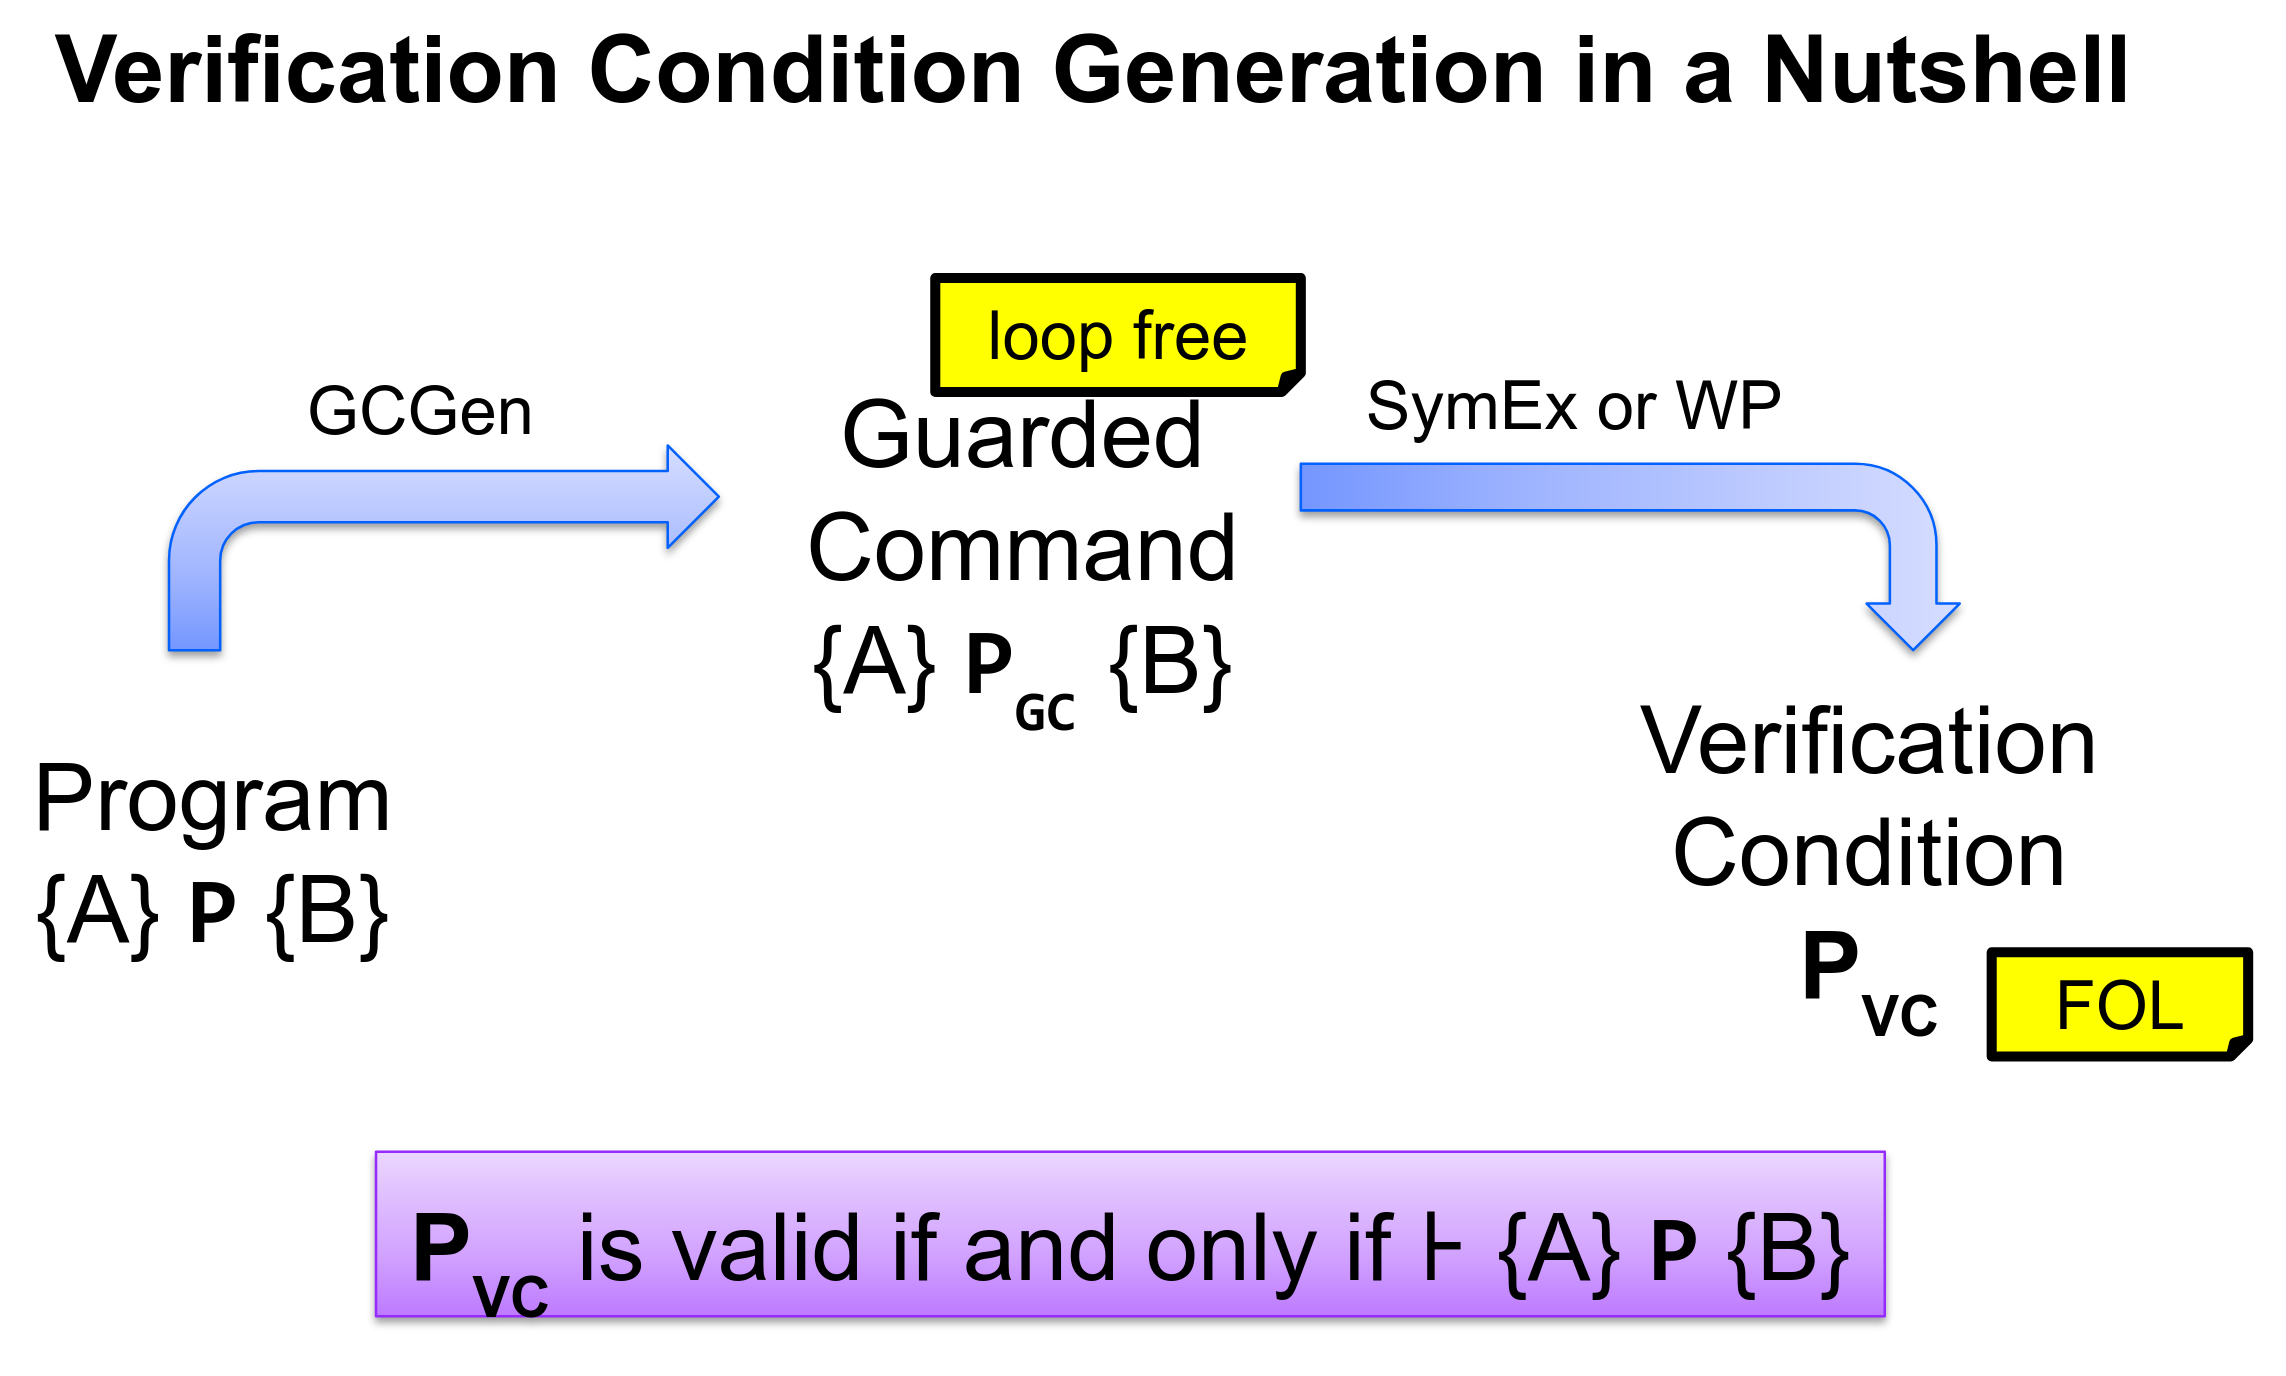
\includegraphics[width=\textwidth]{L17/vcgen.png}

\subsection*{Step 1: Loop-Free Guarded Commands}
For verification purposes, we first compile the program into loop-free guarded commands.
Here's the grammar for these commands.

\begin{verbatim}
c ::= assume b
  |   assert b
  |   havoc x
  |   c1; c2
  |   c1 || c2
\end{verbatim}
The guards are the asserts and assumes. You can't execute a program once it's been compiled to guarded commands,
but proving correctness of the guarded commands is equivalent to proving correctness of the original.

Let's look at the rules to translate WHILE into guarded commands. This is similar to Hoare Logic.
\begin{itemize}[noitemsep]
\item GC(\textsf{skip}): \textsf{assume true}
\item GC(\textsf{x := e}): \textsf{assume tmp = x; havoc x; assume (x = e[tmp/x])}, where \textsf{tmp} is fresh.
\item GC($\mathsf{c}_1; \mathsf{c}_2$): GC($\mathsf{c}_1$); GC($\mathsf{c}_2$)
\item GC(\textsf{if $b$ then c$_1$ else c$_2$}): (\textsf{assume $b$;} GC($\mathsf{c}_1$) $\mid \mid$ \textsf{assume $\neg b$;} GC($\mathsf{c}_2$)
\item GC(\textsf{while $b$ inv I do c}): \ldots
\end{itemize}

The rule for assignment is like the one for Hoare Logic. We zero out \textsf{x} and then assume that it is \textsf{e}, taking care to not use the \textsf{x} that we're defining if it should occur in \textsf{e}, but rather old \textsf{x}.

For \textsf{if}, it looks like we have parallel composition, but in any actual execution, either $b$ is concretely true or concretely false. So one of the branches has what amounts to \textsf{assume false} and verification would stop on that branch in that condition. The execution continues on the branch that does not have an \textsf{assume false}.

We've also seen the translation for loops:
\begin{itemize}[noitemsep]
\item GC(\textsf{while $b$ inv I do c}): \\
\hspace*{2em}
  \begin{minipage}{.8\textwidth}
    \textsf{assert I;} \\
    \textsf{havoc $x_1$; \ldots; havoc $x_n$;} \qquad \qquad // (variables modified in \textsf{c})\\
    \textsf{assume I;} \\
    \textsf{((assume $b$; }GC\textsf{(c); assert I; assume false) $\mid \mid$} \\
    \textsf{\hspace*{1em} assume $\neg b$)}
  \end{minipage}
\end{itemize}

\newpage
\paragraph{Example.} Let's look at how this works on our multiplication example again.
\begin{lstlisting}
{n >= 0} 
p := 0; 
x := 0; 
while x < n inv p = x * m && x <= n do 
  x := x + 1; 
  p := p + m
{p = n * m}
\end{lstlisting}
The conversion is mechanical and we get this:
\begin{lstlisting}
{ n >= 0 }
assume p0 = p; havoc p; assume p = 0; 
assume x0 = x; havoc x; assume x = 0; 
assert p = x * m && x <= n;
havoc x; havoc p; assume p = x * m && x <= n;
  ((assume x < n; 
    assume x1 = x; havoc x; assume x = x1 + 1; 
    assume p1 = p; havoc p; assume p = p1 + m; 
    assert p = x * m && x <= n; assume false) 
   || assume x >= n)
{ p = n * m }
\end{lstlisting}
For the assignment statements, we can see both the cases where there is no capture and where an assignment
refers to the old value of, for instance, \texttt{x}---it introduces temporary variable \texttt{x1}.
For the while loop, we assert the invariant before the loop, then clear everything but the invariant, assume it,
and show it at the end of the loop body. When exiting the loop, we assume the negation of the loop body.

\subsection*{Step 2: Verification Condition Generation}
Here are two ways we could proceed.

\paragraph{Idea 1: Exhaustive symbolic execution of GC program.}
We've seen symbolic execution. It is, in principle, possible to use it to verify the guarded commands:
start at the beginning, keep on tracking the symbolic state, and see if we can prove the postcondition at the end.
The program is correct if no assertion can fail.

The symbolic execution is implicitly constructing verification conditions and bringing them through to the end.

Because of the way this works, we start with the pre-condition, and use the program structure, but here we are
bringing \emph{everything} through to the end, even if that is much more than what is needed to prove the postcondition.
The symbolic state, for instance, can get exponentially huge, and we'd rather not have that.

\paragraph{Idea 2: Propagate the post-condition backwards through the program.} Here, the idea is to use the post-condition
and proceed backwards, checking that the required pre-condition, plus the program behaviour, is strong enough to ensure
the post-condition.

That is, for a Hoare triple
$\{ A \} P \{ B \}$, we generate FOL formula $A \Rightarrow F(P, B)$, where backwards propagation $F(P, B)$ is formalized
in terms of \emph{weakest preconditions}.

This approach has always seemed less intuitive to me than the symbolic execution approach, but it does work better.

The weakest precondition $\mathrm{WP}(c, B)$ holds for any state $q$ whose $c$-successor states
all satisfy $B$; that is,
\[
q \models \mathrm{WP}(c, B) \mathrm{~~~iff~~~} \forall q' \in Q. ~q \xrightarrow{c} q' \Rightarrow q' \models B
\]

Or, as a picture:
\begin{center}
  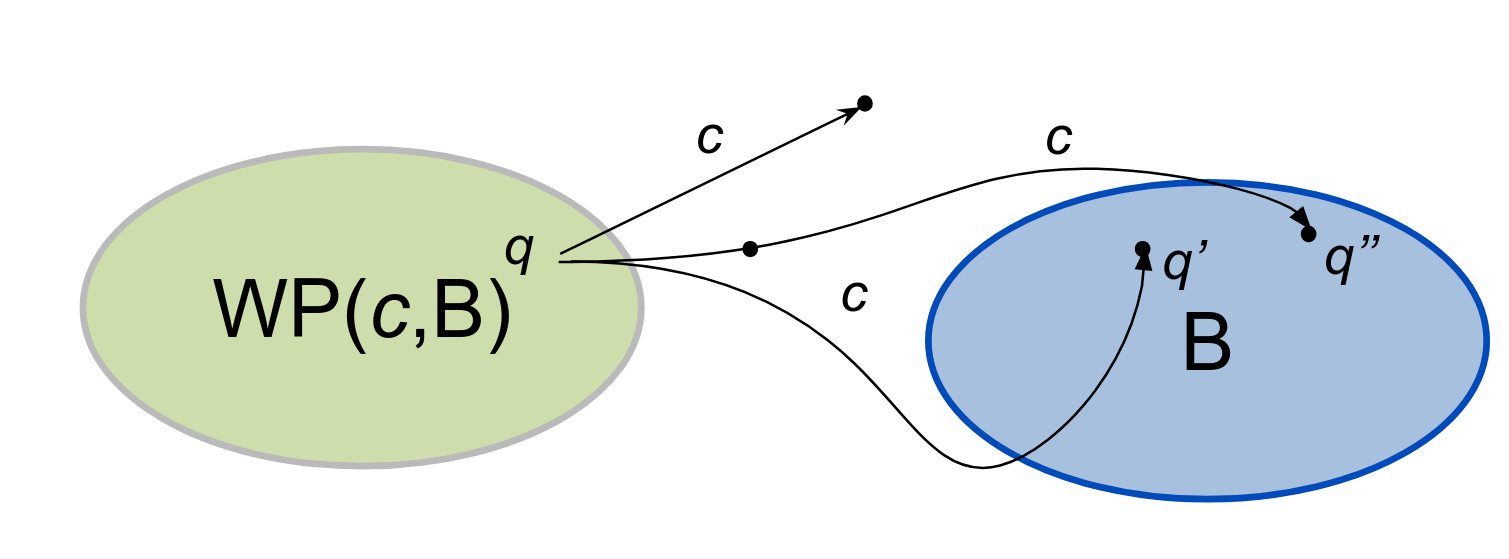
\includegraphics[width=.6\textwidth]{L17/wp.png}
\end{center}
It really is backwards, but effective.

\paragraph{WP Examples.} Let's again work through some examples. This is similar to the Hoare Logic examples we saw earlier. It's a mechanical process
to start with, but then also we can simplify the formulas.

\[
\begin{array}{lll}
  \{ \hspace*{5em} \} & x := z + w &\{ x \geq y \} \\
  \{ \hspace*{5em} \} & \mathsf{if~}y > 0\mathsf{~then~} x := x + 1 \mathsf{~else~} x := y + 4 &\{x \geq 42 \} \\
  \{ \hspace*{5em} \} & \mathsf{if~}y > 0\mathsf{~then~} x := z \mathsf{~else~} x := y &\{ x \geq y + z \} \\
\end{array}
\]

For the first one, we push through the RHS to obtain weakest precondition
\[ z + w \geq y \]
If you think about it for a bit---or, better yet, work through some examples---you can see that anything weaker is not going to give the needed postcondition, but that what we have here does.

We can mechanically push backwards $x \geq 42$ in the second case, getting a disjunction:
\[ (y > 0 \wedge x + 1 \geq 42) \vee (y \leq 0 \wedge y + 4 \geq 42) \]
which simplifies to
\[ (y > 0 \wedge x \geq 41) \vee (y \leq 0 \wedge y  \geq 38) \]
and we can drop the second disjunct, which can never be true, to get weakest precondition:
\[ y > 0 \wedge x \geq 41 \]

Similarly, in the third case, the mechanical process yields:
\[ (y > 0 \wedge z \geq y + z) \vee (y \leq 0 \wedge y \geq y + z) \]
which simplifies to
\[ (y > 0 \wedge 0 \geq y) \vee (y \leq 0 \wedge 0 \geq z) \]
also known as
\[ (y = 0) \vee (y \leq 0 \wedge z \leq 0) \]
This is all mechanical and Dafny does it for you.

So, now we can compute weakest pre-conditions. How does that help for program verification?
We have a method, along with a post-condition, and compute the weakest pre-condition.
If the method pre-condition is stronger than the weakest pre-condition, then any valid
way that you call the method is going to ensure the stated post-condition. This verifies
the method.

(Another way of saying this is that, if you put the pre-condition as an assume at the
beginning of the method, then you have to compute the weakest pre-condition as \textsf{true};
otherwise, anything that is ``left over'' is a way to break the function contract.)

\paragraph{Computing Weakest Pre-conditions.} Here are rules for mechanically computing
the weakest preconditions.

\begin{itemize}[noitemsep]
\item WP(\textsf{assume }$b$, $B$): $b \Rightarrow B$
\item WP(\textsf{assert }$b$, $B$): $b \wedge B$
\item WP(\textsf{havoc }$x$, $B$): $B[a/x]$ \hspace*{5em} ($a$ fresh in $B$; ``replace $x$ by $a$'')
\item WP($c_1$~;~$c_2$, $B$): WP($c_1$, WP($c_2$, $B$))
  \item WP($c_1 \mid\mid c_2$, $B$): WP($c_1$, $B$) $\wedge$ WP($c_2$, $B$)
\end{itemize}

Let's start with $c_1 \mid\mid c_2$. In that case, the weakest precondition has to be the conjunction of those for $c_1$ and $c_2$, because either of those
(or both, in some sense) could execute, so we'd better account for them.

Conversely, for sequential composition, we calculate the WP for $c_2$ first, and then take its output, go backwards, and compute the weakest precondition for
$c_1$. So you can get to the start of $c_1$ by going through $c_2$ and then $c_1$.

For a \textsf{havoc} statement, we wipe out everything we knew about $x$ and put in some fresh $a$ to replace it. $B$ has to be true no matter what $x$ is afterwards. The new $a$ can pick up more constraints
as the computation continues backwards through the method.

The weakest precondition for an \textsf{assert} is that the expression $b$ being asserted must hold as part of the weakest precondition. Otherwise, the execution aborts. Note that this doesn't change the state.

Finally, for an \textsf{assume} statement, we use the property of implication where we make no guarantees about what happens if the antecedent is false.
So, if the antecedent is true (the assumption holds), then we say the incoming thing $B$; otherwise, we basically quietly abort the execution and pretend nothing happened. (There is a subtle point about partial correctness here; the requirement is just that there \emph{exists} an execution that has the desired effect, not that all executions do, so \textsf{assume} can drop executions and it's fine.)

\paragraph{Putting everything together.} This is what Dafny does:

Given a Hoare triple $H \equiv \{ A \} P \{ B \}$,
\begin{itemize}[noitemsep]
\item compute $c_H := \mathsf{assume~}A; ~\mathrm{GC}(P); \mathsf{assert~}B$;
\item compute $\mathrm{VC}_H := \mathrm{WP}(c_H, \mathsf{true})$; and,
\item prove $\vdash \mathrm{VC}_H$ using a theorem prover.
\end{itemize}

\paragraph{One last example.} But it's a bit of a doozy. Let's compute the weakest precondition of the multiplication program, which we'd already converted to the guarded command language.

\begin{Verbatim}[commandchars=\\\{\}]
  WP( assume n \(\geq\) 0;
      assume p0 = p; havoc p; assume p = 0; 
      assume x0 = x; havoc x; assume x = 0; 
      assert p = x * m \(\wedge\) x \( \leq \) n;
      havoc x; havoc p; assume p = x * m \(\wedge\) x \( \leq \) n;
          ((assume x < n; 
            assume x1 = x; havoc x; assume x = x1 + 1; 
            assume p1 = p; havoc p; assume p = p1 + m; 
            assert p = x * m \(\wedge\) x \( \leq \) n; assume false) 
          || assume x \(\geq\) n) ;
      assert p = n * m, true)
\end{Verbatim}
We have incorporated the precondition and postcondition already, as an assume/assert pair, so we aim to finish with weakest precondition \textsf{true}.

We start at the end with the \textsf{assert} statement, which got tacked on to the end using sequential composition. WP for the assert is \texttt{p = n * m} and
applying the rule for \verb+;+ gives us new $B$ being the same expression:
\begin{Verbatim}[commandchars=\\\{\}]
  WP( assume n \(\geq\) 0;
      assume p0 = p; havoc p; assume p = 0; 
      assume x0 = x; havoc x; assume x = 0; 
      assert p = x * m \(\wedge\) x \(\leq\) n;
      havoc x; havoc p; assume p = x * m \(\wedge\) x \(\leq\) n;
          ((assume x < n; 
            assume x1 = x; havoc x; assume x = x1 + 1; 
            assume p1 = p; havoc p; assume p = p1 + m; 
            assert p = x * m \(\wedge\) x \(\leq\) n; assume false) 
          || assume x \(\geq\) n), p = n * m)
\end{Verbatim}
Continuing backwards, the next sequential composition is between
\begin{Verbatim}[commandchars=\\\{\}]
  assume p = x * m \(\wedge\) x \(\leq\) n
\end{Verbatim}
and what we got converting the \textsf{while} body, so we split this and
compute the weakest preconditon of the loop body separately; it'll be the input to computing
WP on everything before that.
\begin{Verbatim}[commandchars=\\\{\}]
  WP( assume n \(\geq\) 0;
      assume p0 = p; havoc p; assume p = 0; 
      assume x0 = x; havoc x; assume x = 0; 
      assert p = x * m \(\wedge\) x \(\leq\) n;
      havoc x; havoc p; assume p = x * m \(\wedge\) x \(\leq\) n,
        WP((assume x < n; 
            assume x1 = x; havoc x; assume x = x1 + 1; 
            assume p1 = p; havoc p; assume p = p1 + m; 
            assert p = x * m \(\wedge\) x \(\leq\) n; assume false) 
          || assume x \(\geq\) n, p = n * m))
\end{Verbatim}
We have a $\mid\mid$, so we change that into a conjunction.
\begin{Verbatim}[commandchars=\\\{\}]
  WP( assume n \(\geq\) 0;
      assume p0 = p; havoc p; assume p = 0; 
      assume x0 = x; havoc x; assume x = 0; 
      assert p = x * m \(\wedge\) x \(\leq\) n;
      havoc x; havoc p; assume p = x * m \(\wedge\) x \(\leq\) n,
        WP(assume x < n; 
            assume x1 = x; havoc x; assume x = x1 + 1; 
            assume p1 = p; havoc p; assume p = p1 + m; 
            assert p = x * m \(\wedge\) x \(\leq\) n; assume false, p = n * m)
      \(\wedge\) WP(assume x \(\geq\) n, p = n * m))
\end{Verbatim}
Let's convert the last \textsf{assume} into an implication.
\begin{Verbatim}[commandchars=\\\{\}]
  WP( assume n \(\geq\) 0;
      assume p0 = p; havoc p; assume p = 0; 
      assume x0 = x; havoc x; assume x = 0; 
      assert p = x * m \(\wedge\) x \(\leq\) n;
      havoc x; havoc p; assume p = x * m \(\wedge\) x \(\leq\) n,
        WP(assume x < n; 
            assume x1 = x; havoc x; assume x = x1 + 1; 
            assume p1 = p; havoc p; assume p = p1 + m; 
            assert p = x * m \(\wedge\) x \(\leq\) n; assume false, p = n * m)
      \(\wedge\) x \(\geq\) n \(\Rightarrow\) p = n * m)
\end{Verbatim}
\newpage
Now for the loop body, where we have another sequential composition with its last \textsf{assume false}:
\begin{Verbatim}[commandchars=\\\{\}]
  WP( assume n \(\geq\) 0;
      assume p0 = p; havoc p; assume p = 0; 
      assume x0 = x; havoc x; assume x = 0; 
      assert p = x * m \(\wedge\) x \(\leq\) n;
      havoc x; havoc p; assume p = x * m \(\wedge\) x \(\leq\) n,
        WP(assume x < n; 
            assume x1 = x; havoc x; assume x = x1 + 1; 
            assume p1 = p; havoc p; assume p = p1 + m; 
            assert p = x * m \(\wedge\) x \(\leq\) n; WP(assume false, p = n * m))
      \(\wedge\) x \(\geq\) n \(\Rightarrow\) p = n * m)
\end{Verbatim}
Let's process the \textsf{assume false} and understand how that stops considering what happens going off the end of the loop body.
\begin{Verbatim}[commandchars=\\\{\}]
  WP( assume n \(\geq\) 0;
      assume p0 = p; havoc p; assume p = 0; 
      assume x0 = x; havoc x; assume x = 0; 
      assert p = x * m \(\wedge\) x \(\leq\) n;
      havoc x; havoc p; assume p = x * m \(\wedge\) x \(\leq\) n,
        WP(assume x < n; 
            assume x1 = x; havoc x; assume x = x1 + 1; 
            assume p1 = p; havoc p; assume p = p1 + m; 
            assert p = x * m \(\wedge\) x \(\leq\) n, false \(\Rightarrow\) p = n * m)
      \(\wedge\) x \(\geq\) n \(\Rightarrow\) p = n * m)
\end{Verbatim}
So now $B$ for the WP for the loop body is $\mathsf{false} \Rightarrow \ldots$: we don't
care what happens after the end of the loop body, we just need to show all the assertions before the end of the loop.
That is,
\begin{Verbatim}[commandchars=\\\{\}]
  WP( assume n \(\geq\) 0;
      assume p0 = p; havoc p; assume p = 0; 
      assume x0 = x; havoc x; assume x = 0; 
      assert p = x * m \(\wedge\) x \(\leq\) n;
      havoc x; havoc p; assume p = x * m \(\wedge\) x \(\leq\) n,
        WP(assume x < n; 
            assume x1 = x; havoc x; assume x = x1 + 1; 
            assume p1 = p; havoc p; assume p = p1 + m; 
            assert p = x * m \(\wedge\) x \(\leq\) n, true)
      \(\wedge\) x \(\geq\) n \(\Rightarrow\) p = n * m)
\end{Verbatim}
Continuing inside the loop body and applying sequential composition and \textsf{assert},
\begin{Verbatim}[commandchars=\\\{\}]
  WP( assume n \(\geq\) 0;
      assume p0 = p; havoc p; assume p = 0; 
      assume x0 = x; havoc x; assume x = 0; 
      assert p = x * m \(\wedge\) x \(\leq\) n;
      havoc x; havoc p; assume p = x * m \(\wedge\) x \(\leq\) n,
        WP(assume x < n; 
            assume x1 = x; havoc x; assume x = x1 + 1; 
            assume p1 = p; havoc p; assume p = p1 + m,
            p = x * m \(\wedge\) x \(\leq\) n)
      \(\wedge\) x \(\geq\) n \(\Rightarrow\) p = n * m)
\end{Verbatim}
We apply another \textsf{assume}:
\begin{Verbatim}[commandchars=\\\{\}]
  WP( assume n \(\geq\) 0;
      assume p0 = p; havoc p; assume p = 0; 
      assume x0 = x; havoc x; assume x = 0; 
      assert p = x * m \(\wedge\) x \(\leq\) n;
      havoc x; havoc p; assume p = x * m \(\wedge\) x \(\leq\) n,
        WP(assume x < n; 
            assume x1 = x; havoc x; assume x = x1 + 1; 
            assume p1 = p; havoc p,
            p = p1 + m \(\Rightarrow\) p = x * m \(\wedge\) x \(\leq\) n)
      \(\wedge\) x \(\geq\) n \(\Rightarrow\) p = n * m)
\end{Verbatim}
Now for the \textsf{havoc} and \textsf{assume}, we introduce fresh variable \texttt{pa1} and substitute it for \texttt{p}:
\begin{Verbatim}[commandchars=\\\{\}]
  WP( assume n \(\geq\) 0;
      assume p0 = p; havoc p; assume p = 0; 
      assume x0 = x; havoc x; assume x = 0; 
      assert p = x * m \(\wedge\) x \(\leq\) n;
      havoc x; havoc p; assume p = x * m \(\wedge\) x \(\leq\) n,
        WP(assume x < n; 
            assume x1 = x; havoc x; assume x = x1 + 1,
            p1 = p \(\wedge\) pa1 = p1 + m \(\Rightarrow\) pa1 = x * m \(\wedge\) x \(\leq\) n)
      \(\wedge\) x \(\geq\) n \(\Rightarrow\) p = n * m)
\end{Verbatim}
Continuing with \texttt{x = x1 + 1}:
\begin{Verbatim}[commandchars=\\\{\}]
  WP( assume n \(\geq\) 0;
      assume p0 = p; havoc p; assume p = 0; 
      assume x0 = x; havoc x; assume x = 0; 
      assert p = x * m \(\wedge\) x \(\leq\) n;
      havoc x; havoc p; assume p = x * m \(\wedge\) x \(\leq\) n,
        WP(assume x < n; 
            assume x1 = x; havoc x,
            x = x1 + 1 \(\wedge\) p1 = p \(\wedge\) pa1 = p1 + m \(\Rightarrow\) pa1 = x * m \(\wedge\) x \(\leq\) n)
      \(\wedge\) x \(\geq\) n \(\Rightarrow\) p = n * m)
\end{Verbatim}
\newpage
and another \textsf{havoc}, introducing fresh \texttt{xa1}:
\begin{Verbatim}[commandchars=\\\{\}]
  WP( assume n \(\geq\) 0;
      assume p0 = p; havoc p; assume p = 0; 
      assume x0 = x; havoc x; assume x = 0; 
      assert p = x * m \(\wedge\) x \(\leq\) n;
      havoc x; havoc p; assume p = x * m \(\wedge\) x \(\leq\) n,
        WP(assume x < n; assume x1 = x,
            xa1 = x1 + 1 \(\wedge\) p1 = p \(\wedge\) pa1 = p1 + m \(\Rightarrow\) pa1 = xa1 * m \(\wedge\) xa1 \(\leq\) n)
      \(\wedge\) x \(\geq\) n \(\Rightarrow\) p = n * m)
\end{Verbatim}
which leaves us with another \texttt{assume x1 = x} to handle; we use $\wedge$ because we are tacking it onto the antecedent of the implication here (essentially, we are simultaneously assuming multiple things).
\begin{Verbatim}[commandchars=\\\{\}]
  WP( assume n \(\geq\) 0;
      assume p0 = p; havoc p; assume p = 0; 
      assume x0 = x; havoc x; assume x = 0; 
      assert p = x * m \(\wedge\) x \(\leq\) n;
      havoc x; havoc p; assume p = x * m \(\wedge\) x \(\leq\) n,
        WP(assume x < n,  
            x1 = x \(\wedge\) xa1 = x1 + 1 \(\wedge\) p1 = p \(\wedge\) pa1 = p1 + m \(\Rightarrow\) pa1 = xa1 * m \(\wedge\) xa1 \(\leq\) n)
      \(\wedge\) x \(\geq\) n \(\Rightarrow\) p = n * m)
\end{Verbatim}
and finally completing the loop body:
\begin{Verbatim}[commandchars=\\\{\}]
  WP( assume n \(\geq\) 0;
      assume p0 = p; havoc p; assume p = 0; 
      assume x0 = x; havoc x; assume x = 0; 
      assert p = x * m \(\wedge\) x \(\leq\) n;
      havoc x; havoc p; assume p = x * m \(\wedge\) x \(\leq\) n,
        x < n \(\wedge\) x1 = x \(\wedge\) xa1 = x1 + 1 \(\wedge\) p1 = p \(\wedge\) pa1 = p1 + m
             \(\Rightarrow\) pa1 = xa1 * m \(\wedge\) xa1 \(\leq\) n
      \(\wedge\) x \(\geq\) n \(\Rightarrow\) p = n * m)
\end{Verbatim}
If we continue through the beginning of the method, we get this formula:
\begin{Verbatim}[commandchars=\\\{\}]
  n \(\geq\) 0 \(\wedge\) p0 = p \(\wedge\) pa3 = 0 \(\wedge\) x0 = x \(\wedge\) xa3 = 0 \(\Rightarrow\)
    pa3 = xa3 * m \(\wedge\) xa3 \(\leq\) n \(\wedge\)
    (pa2 = xa2 * m \(\wedge\) xa2 \(\leq\) n \(\Rightarrow\)
      ((xa2 \(<\) n \(\wedge\) x1 = xa2 \(\wedge\) xa1 = x1 + 1 \(\wedge\) p1 = pa2 \(\wedge\) pa1 = p1 + m) \(\Rightarrow\)
          pa1 = xa1 * m \(\wedge\) xa1 \(\leq\) n
      ) \(\wedge\)
      (xa2 \(\geq\) n \(\Rightarrow\) pa2 = n * m)
    )
\end{Verbatim}
\newpage
which is equivalent to the conjunction of the three formulas, representing the three things to prove for a loop:
\begin{Verbatim}[commandchars=\\\{\}]
  n \(\geq\) 0 \(\wedge\) p0 = p \(\wedge\) pa3 = 0 \(\wedge\) x0 = x \(\wedge\) xa3 = 0 \(\Rightarrow\)
    pa3 = xa3 * m \(\wedge\) xa3 \(\leq\) n

  n \(\geq\) 0 \(\wedge\) p0 = p \(\wedge\) pa3 = 0 \(\wedge\) x0 = x \(\wedge\) xa3 = 0 \(\wedge\) pa2 = xa2 * m \(\wedge\) xa2 \(\leq\) n \(\Rightarrow\)
   (xa2 \(\geq\) n \(\Rightarrow\) pa2 = n * m)

  n \(\geq\) 0 \(\wedge\) p0 = p \(\wedge\) pa3 = 0 \(\wedge\) x0 = x \(\wedge\) xa3 = 0 \(\wedge\) pa2 = xa2 * m \(\wedge\) xa2 \(\leq\) n \(\wedge\)
   x1 = xa2 \(\wedge\) xa1 = x1 + 1 \(\wedge\) p1 = pa2 \(\wedge\) pa1 = p1 + m \(\Rightarrow\) pa1 = xa1 * m \(\wedge\) xa1 \(\leq\) n
\end{Verbatim}
with the first condition being that the loop invariant holds upon entry; the second that it implies the postcondition; and the third that it is preserved by the loop body.

It is possible to simplify these constraints to (or just feed them as-is to a solver):
\begin{Verbatim}[commandchars=\\\{\}]
  n \(\geq\) 0 \(\Rightarrow\) 0 = 0 * m \(\wedge\) 0 \(leq\) n

  xa2 \(\leq\) n \(\wedge\) xa2 \(\geq\) n \(\Rightarrow\) xa2 * m = n * m

  xa2 \(<\) n \(\Rightarrow\) xa2 * m + m = (xa2 + 1) * m \(\wedge\) xa2 + 1 \(\leq\) n
\end{Verbatim}
which are all valid, proving that the original Hoare triple was also valid.


\end{document}
